\documentclass{article}
\usepackage{amsmath}
\usepackage{amssymb}
\usepackage{graphicx}
\usepackage{hyperref}
\usepackage[version=4]{mhchem}

\title{Example 6}
\date{}

\begin{document}
\maketitle

Triangle \(A B C\) is inscribed in the circle \(O\). The diameter \(B D\) meets \(A C\) at \(E\). Draw \(A F \perp B D, F\) is the foot of the perpendicular from \(A\) to \(B D\). Extend \(A F\) to meet \(B C\) at \(G\). Show that \(A B^{2}\) \(=B G \times B C\).

Solution:
Connect \(A D\). Since points \(A, B, C\), and \(D\) are concyclic,\\
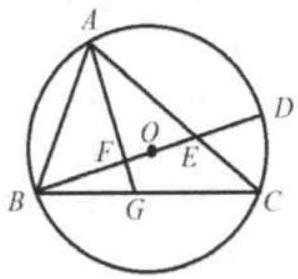
\includegraphics[width=\textwidth]{images/165(4).jpg} \(\angle C=\angle D\).\\
Since \(B D\) is the diameter, \(\angle B A D=90^{\circ}\).\\
\(\angle D=90^{\circ}-\angle A B D\).\\
Since \(A F \perp B D\), in Rt \(\triangle B A F, \angle B A F=90^{\circ}-\angle A B D\).\\
\centering
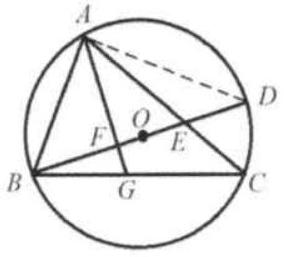
\includegraphics[width=\textwidth]{images/165(2).jpg}

Thus \(\angle C=\angle B A F\).\\
Since \(\angle A B C=\angle A B G, \triangle A B G \sim \triangle C B A\).\\
Thus \(\frac{A B}{C B}=\frac{B G}{B A} \quad \Rightarrow \quad A B^{2}=B G \times B C\).\\
\centering
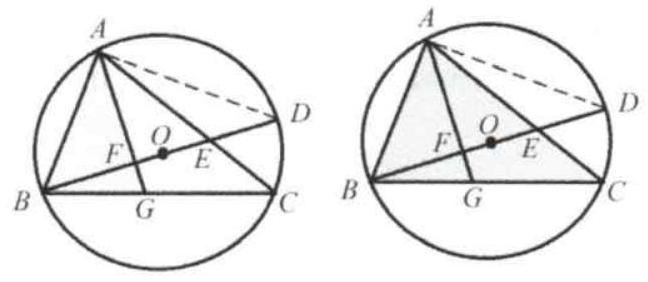
\includegraphics[width=\textwidth]{images/166.jpg}


\end{document}
